\documentclass[10pt,journal,final,letterpaper,twocolumn]{IEEEtran}
%\documentclass{ssdbm}
\usepackage{wrapfig,subfigure,setspace,verbatim,cite,url,graphicx,float}
\usepackage{algorithmic,amsfonts,amssymb,amsmath,calc,calrsfs,cleveref}
\usepackage{epstopdf}
%\usepackage{fixltx2e}

\restylefloat{table}

% This was from the NEW paper
%----------------------------------------------------------
\RequirePackage{fix-cm}

\DeclareMathOperator{\var}{var}
\newcounter{qcounter}

%\smartqed  % flush right qed marks, e.g. at end of proof



%----------------------------------------------------------


\newtheorem{theorem}{Theorem}
\newtheorem{lemma}{Lemma}
\newtheorem{definition}{Definition}
\newtheorem{remark}{Remark}

\newcommand{\SEC}[1] {Section \ref{#1}}
\newcommand{\Eq}[1] {Equation \ref{#1}}
\newcommand{\eq}[1] {Eq. (\ref{#1})}

% correct bad hyphenation here
\hyphenation{op-tical net-works semi-conduc-tor}


\begin{document}


% paper title
\title{Parallelization of Push-based System for Molecular Simulation Data Analysis}

% author names and IEEE memberships
% note positions of commas and nonbreaking spaces ( ~ ) LaTeX will not break
% a structure at a ~ so this keeps an author's name from being broken across
% two lines.
% use \thanks{} to gain access to the first footnote area
% a separate \thanks must be used for each paragraph as LaTeX2e's \thanks
% was not built to handle multiple paragraphs

\author{Iliiazbek~Akhmedov, Yi-Cheng~Tu~$\dagger$% <-this % stops a space

%\thanks{* These authors contributed equally to this work.}
\thanks{$\dagger$ Author to whom all correspondence should be sent.}
\thanks{Vladimir Grupcev and Yi-Cheng Tu are with the Department of Computer
Science and Engineering, University of South Florida, 4202 E. Fowler
Ave., ENB 118, Tampa, FL 33620, U.S.A. Emails:
vgrupcev@mail.usf.edu, ytu@cse.usf.edu}
\thanks{Joseph Fogarty and Sagar Pandit are with the Department of Physics,
University of South Florida, 4202 E. Fowler Ave., ISA 2019, Tampa,
FL 33620, U.S.A. Emails: jcfogart@mail.usf.edu, pandit@usf.edu} }

%\pubid{0000--0000/00\$00.00~\copyright~2002 IEEE}

% use only for invited papers
%\specialpapernotice{(Invited Paper)}

% make the title area
\maketitle

\begin{abstract}

Thanks to the advancement of the modern computer simulation systems
and state-of-the-art instrumentation, many scientific fields
generate, and require manipulation of large amounts of data. Known
scientific data analysis systems, as well as traditional DBMSs,
follow a pull-based type of architectural design, where the executed
queries mandate the data needed on their part. This design, while
suitable for traditional transaction-based workloads where number of
queries retrieve small parts of data located at various places of
the database, is ill-fitted for applications involving complex
analysis on most of the data. Such design involves random I/O,
considerably affecting the data throughput in the system. All of
this gives rise of redundant and high I/O traffic in the process of
scientific data analysis in pull-based type systems. In this paper,
we design and implement a push-based type system which allows
high-throughput data analysis in the process of scientific
discovery. Our design improves on the aforementioned shortcomings in
two ways: i) it uses a sequential scan-based I/O framework that
loads the data into the main memory, and then ii) the system pushes
the loaded data to a number of pre-programmed queries. These queries
are being executed on the same data stream, with various data
selections. This way, essentially, the system lowers the unnecessary
I/O overhead imposed by the randomized, index-based scan and that of
a multiple data reads if each query were to be fed separately.
Considering the amount of MS data as well as the number of queries
being executed, we believe our system provides substantial
improvement over the current MS data analyzing systems. The
efficiency of the proposed system is backed by the results of
extensive experiments using MS generated data. The running times of
our system are compared to those of the GROMACS system. The
comparison shows the advantage and the potential of using such
push-based system for MS system analysis.

\end{abstract}

\begin{IEEEkeywords}
Push-based system, molecular simulation, scientific databases,
spatial distance histogram.
\end{IEEEkeywords}
%\vspace{-5mm}

\begin{comment}
Many scientific applications share several features that bring in
light the shortcomings of the current data analysis systems. First,
the scientific analysis often involves executing a number of
analytical queries commonly processed on a large portion, if not all
of the generated data. Second, many of these fields use the same
popular, and small number of data analytics primitives as the basic
blocks on which they build their discovery. And three, the
scientific data, once stored is never modified. New data only
appends to the existing dataset, making the data perfect contender
for streaming.

And while the use of an index-based scan might seem better option to
a sequential scan, this is the case only when the query accesses
small portion of the data.
\end{comment}

%%%%%%%%%%%%%%%%%%%%%%%%%%%%%%%%%%%%%%%%%%%%%%%%%%%%%%%%%%%%%%%%%%%%%%%%%%%%%%%

\section{Introduction}\label{sc:intro}
The amount of data generated by scientific applications running on
advanced computer simulation systems as well as the new improved
experimental devices is growing rapidly. This big volume of data is
imposing a significant stress on the data analysis software. Even
though the existing data analysis systems are configured to deal
with large volume of data, they are not optimized for high
throughput data analysis. Often times, the data is available only
for certain period of time (e.g., streams) so the analyzing system
should react to it in a very efficient way. On top of the big amount
of data, another challenge that is being imposed to the data
analysis systems is that the data is usually being accessed through
high-level analytical queries which computation is a lot more
complex than the computation of simple aggregates. Some of these
queries are usually the bottleneck of the data analysis systems,
because they take a lot of time (often many days) to be executed and
the systems are not designed to handle multiple queries on the same
data stream at the same time, thus decreasing the overall efficiency
of the data analysis.

One such example, where fast data analysis is crucial involves
online social
media~\cite{nature_bigdata08,nature_bigdata12,science_social10}. The
social media is known to be used for real-time feedback collection,
which is usually associated to a particular topic or
product~\cite{jcs_twitter11}. In order for a system to be able to
perform analytical examination of the data produced in such
streaming media, the system should have the capability of fast data
access. The reason, the millions of data records(tweets) produced
every second~\cite{tkde_big14}. Moreover, these tweets may have
different geographical origin, introducing different languages and
forms and often times containing unsolicited messages, errors,
malicious content, etc. Therefore, some low level data uniformity
and cleaning on top of the data access and management issues should
be considered and possibly incorporated in the process of analytical
investigation in order to achieve relevant result.

The aforementioned big data imposed issues are also frequently
present in many other application fields, e.g., scientific data
analysis. In many scientific and engineering fields, the main
computational method for analyzing physical/chemical attributes of
natural systems is the particle simulation. Such simulations, when
performed in the field of structural and molecular biology, are
commonly called Molecular Simulations. Molecular simulations (MS)
(sometimes called Molecular Dynamics (MD) simulations) are computer
simulations of complex biological, physical or chemical structures.
These simulations, based on some basic theoretical models are widely
utilized as a basic research mechanism for studying the behavior of
the natural systems. The basic units of such systems/simulations are
natural particles (such as atoms, molecules, stars, etc.) and they
interact among each other for a certain period of time following
postulated classical forces. The number of these basic units taking
part in the simulations is big, usually in the range of hundreds of
thousands to millions. For instance, Fig.~\ref{fg:snap-white} shows
a snapshot of a collagen fiber, consisting of $890,000$ particles.
And oftentimes, the simulations produce datasets consisting of more
than one snapshot (frame) of the system's current state at various
time instants. Each of these frames contain all the particles,
together with all their measurements, such as spatial coordinates,
mass, charge, velocity, forces, etc. And usually, a big number of
such frames (in the tens of thousands) are being produced and stored
in the course of a typical simulation. Quantities measured during
the simulations are analyzed to test the theoretical
model~\cite{Frenkel:api01,Landau:cup05}. In short, the MS is proven
and powerful tool for understanding the inner-workings of a
biological system, by supplying a model description of the
biophysical and biochemical processes that are being unfold at a
nanoscopic scale.

In order to achieve objective discovery and to explain the workings
of the scientific systems, scientist must analyze the data produced
by the MS. These analysis oftentimes comprise of computation of very
complex quantities that show statistical properties of the data.
Such queries are of great importance to scientist because they are
the basic assembly blocks for a series of critical quantities needed
to outline the scientific systems \cite{Frenkel:api01}. The methods
by which the data is being accessed as well as these queries are
executed can either increase or decrease the efficiency of an data
analysis system. The known data analysis systems (e.g., Gromacs
\cite{Gromacs-online}) uses pull based type design in which the data
is being fed to the queries only by demand. When a query needs the
data, it requests it, the data is pulled through the system and
delivered to the query. This type of design, we believe, introduces
two types of problematic issues: 1. overhead in I/O traffic by not
allowing for multiple queries to be executed on the same stream of
data at the same time, and 2. cpu/data latency incurred when a
request for the data is sent to the system (the time it takes from a
request to the time the query can actually use the data).


We believe that by using a push-based type system we can remedy such
issues. In the push-based design the queries do not request the
data. Rather, the data is pushed onto the queries automatically and
is being processed by the active queries. This alleviates the I/O
traffic overhead as well as the cpu/data latency incurred for each
query that would have been introduced by a pull-based design. Such a
system design is especially suitable for many scientific
applications which share the following features. First, the
scientific analysis often involves executing a number of analytical
queries commonly processed on a large portion, if not all of the
generated data. Second, many of these fields use the same popular,
and small number of data analytics primitives as the basic blocks on
which they build their discovery. And three, the scientific data,
once stored is never modified. New data only appends to the existing
dataset, making the data perfect contender for streaming.


In this paper, we describe the idea, design and implementation of
such a push-based system. We would like to point out that the work
presented in this paper is an application of such push-based
strategy that has been previously considered in the database
community in the works presented in~\cite{DataPath,Volcano,Qpipe},
as well as the idea of sharing same tuple of data or data scans
across many queries previously introduced
in~\cite{Candea,PredictablePerformance,CooperativeScans}.

To summarize, data-intensive applications often require compelling
amount of storage space and intensive processing capability, but
also need fast data access and high throughput data analysis.
Therefore, the need of a system that will be optimized to access
data fast, with high throughput, as well as efficiently execute the
analytical queries with a possibility of running multiple queries on
the same data stream is of a great importance to the scientific
community.

\begin{figure}
 \centerline{ 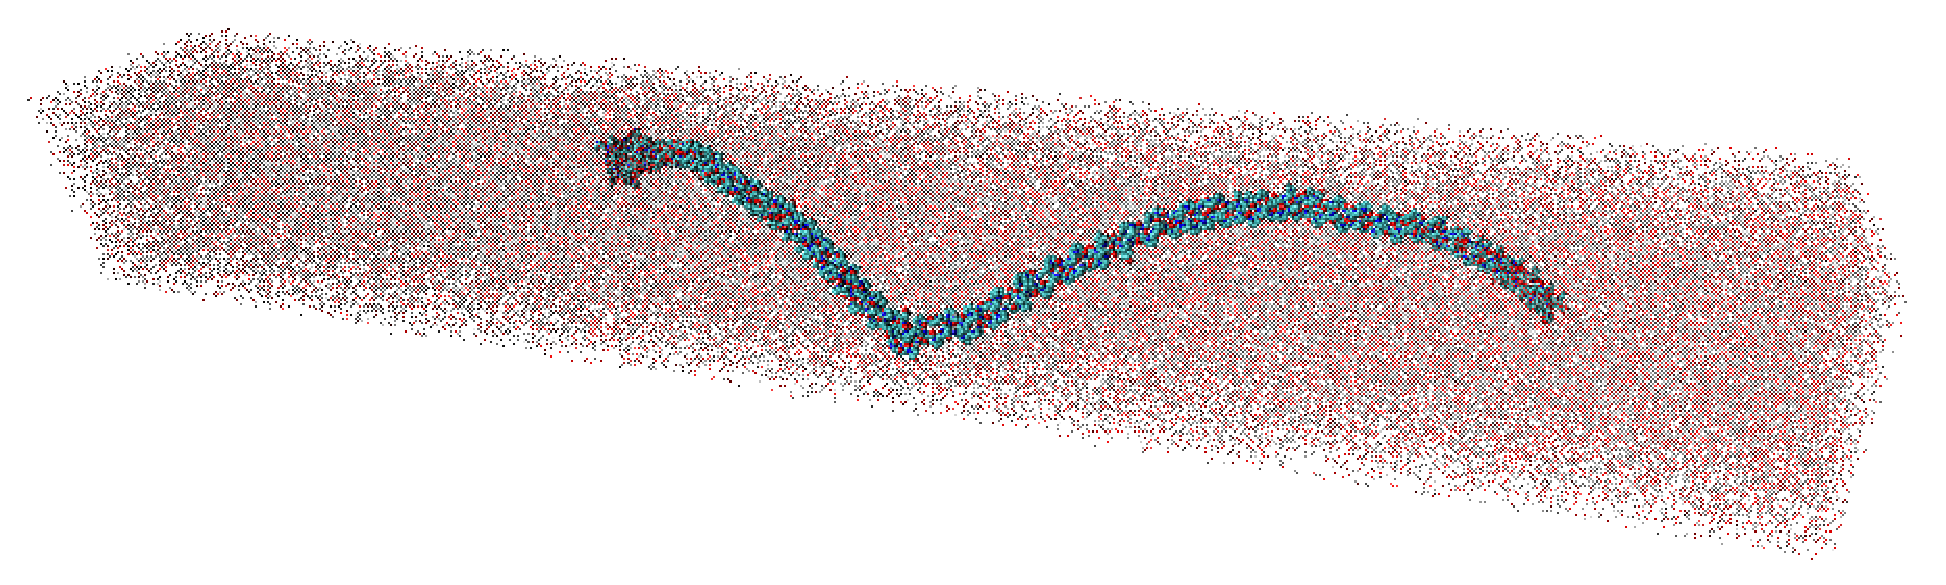
\includegraphics[width=1\columnwidth]{images/snap-white.eps} }
 \caption{A snapshot of simulated collagen fiber structure}
 \label{fg:snap-white}
\end{figure}

\subsection{Problem Statement}
As mentioned earlier, in order to describe the scientific system,
scientist must look into/analyze the critical statistical properties
of the data produced by the simulation. These properties are usually
computed through series of queries that are being executed on the
whole, or some selection of the MS data. Most of the systems that
are widely used today across many scientific fields for analysis of
the MS data are part of a software systems that also run the
simulation. Such examples include GROMACS~\cite{GROMACS4},
VMD~\cite{VMD}, MDAnalysis~\cite{MDAnalysis}, Wordom~\cite{wordom},
MD-TRACKS~\cite{MDtracks}, SimulaidOne~\cite{Simulaid},
Charmm~\cite{CHARMM}. Once the simulation is run, the system
produces a flat file with all the measurements of each particle.
These systems take each query as a user's input and apply them to
the data uploaded from these flat files (called trajectories in
GROMACS). The biggest problem/performance issue that these system
impose is the fact that for every new query issued by the user, the
system has to load a significant part of the dataset into main
memory before executing the query. Such pull-based design involves
random I/Os that considerably affecting the data throughput in the
system. And while the use of an index-based scan might seem better
option to a sequential scan, this is the case only when the query
accesses small portion of the data. All of this gives rise of
redundant and high I/O traffic in the process of scientific data
analysis in pull-based type systems. This adds greatly to the
overall performance time of the analysis of the MS system. Having in
mind the volume of data produced by the MS in a single frame (in
gigabytes), and we add the number of frames simulated (tens of
thousands) the total volume of data to be analyzed is of huge
magnitude. So to have to load big chunks of this data from disk to
the main memory every time a query is being executed degrades the
overall system's performance greatly. In this paper we design and
implement a push-based type system which allows high-throughput data
analysis in the process of scientific discovery.

\subsection{Our Approach}
Considering the fact that the running time of the most queries used
in the scientific world to analyze the MS is minuscule in comparison
to the loading time of the MS data, it is safe to say that the
scientific world would benefit from a system that can remedy the
aforementioned problem. Our idea is to build a system that would
load the MS data from hard disk in the main memory only once and
then execute as many queries as needed/wanted on that data, without
the need of reloading the same data over and over again. Considering
the volume of data in a single MS frame as well as the number of
frames produced during a single simulation, this type of system can
save a lot of time for MS analysis. The system would contain many,
most often used queries that can also be run as user's input. These
queries would be pre-programmed as separate modules in our system,
but they would be able to take certain attributes, like data
selection for instance, as user's input. Once the system is run, all
(or a selection) of these queries would be executed against the MS
data or certain selection. The system would act as a type of
push-based system, essentially pushing the loaded data to all the
queries. Once we have the data in the memory, the reading can loop
as many times as the queries need it. This is useful for some
non-streaming functions/queries that cannot be computed in a single
run of the data. Such one query is the SDH. But we have also come up
with a way to resolve this in a way, by creating a quad-tree based
database for this query. This quad-tree (we called Density Map (DM))
is being populated while the data is being loaded into main memory.
After the DM is populated, we can compute the SDH with much faster
algorithm than the brute-force method used everywhere else.

Another improvement that our system provides is the following: by
thorough observation and analysis we have discovered that many of
the quantities (functions/queries) that are being computed in order
to analyze the MS system share some of the same basic parts. In
order to take advantage of that, our systems precomputes these basic
parts and has them handy (stored in memory) whenever one of the more
complex functions needs them. So, for instance, when the total mass
of the system is needed, our system just pulls the precomputed value
out and serves the query that needs it immediately. And if more than
one query uses the same basic part, that translates into time
saving, however minuscule it might be.

\subsection{Contribution and roadmap of the paper} We have designed
and implemented a push-based system that can be used as a tool for
analysis of MS systems. We have tested the system on real MS
datasets. The experimental results evidently show the superiority of
the proposed system over one of the most widely used MS analysis
system across many scientific fields, i.e., GROMACS. The efficiency
improvement ranges anywhere from $3$ to $100$ times improvement (of
the overall running time) per set of selected queries run on a
different selection of the MS data. If we take in account the number
of such queries that the scientist run every day, we believe our
system would be of great benefit to MS community. In addition to the
higher efficiency that our system achieves, we also believe that our
idea will initiate a new breed of database related, push-based
systems that could be used to analyze the MS systems in a more
efficient way. Having a push-based like system, we were also able to
improve the computation of the more complex quantities. Namely, the
computation of some such complex quantities involves computation of
much less complex functions (sub-parts), and many such sub-parts are
being shared among some of the complex quantities. So, by computing
these more basic, sub-quantities in advance, we were able to achieve
however minuscule time gain when computing the more complex queries.

The major technical contributions presented here are:
\begin{itemize}
\item Design the network (tree like) of the most commonly used queries in MS (physics);
\item Build the system: design and build the modules, representing the quantities to be
computed in an efficient manner, following the already built
network;
\item Develop a scientific simulation database benchmark that can be used for evaluating similar systems and products.
\end{itemize}

The remainder of this paper is arranged as follows: in Section
\ref{sc:relatedwork} we give a survey of the systems used in the
field of MS systems analysis. We continue the paper with Section
\ref{sc:querynetwork} in which we show the design of the query
network build from the most widely used quantities in MS system
analysis. In Section \ref{sc:system} we describe our push-based
system for MS data analysis. Then, in Section \ref{sc:experiments}
we present the benchmark designed to test our system as well as the
results attained through comprehensive experiments run on real MS
generated data. At the end, we conclude this paper with Section
\ref{sc:conclusion} in which we give an overview of our possible
future endeavors in the field of MS data analysis.


%%%%%%%%%%%%%%%%%%%%%%%%%%%%%%%%%%%%%%%%%%%%%%%%%%%%%%%%%%%%%%%%%%%%%%%%%%%%%%%


\section{Related Work}\label{sc:relatedwork}
The idea of data streaming has been broadly used in many fields. The
main usage however is aimed at processing live data generated
online. There is an ocean of references for data stream management,
but we believe the presentation in~\cite{DataStreamManagement}
encapsulates the majority of the ideas, problems and solutions. In
the past decade, however, the database community started to follow
the data stream idea to process stored data. Processes can take
advantage of the streaming data at any time the data is being pushed
through the system. This gives rise to push-based type design for
data management systems. The idea of such push-based design was
previously considered in projects such as DataPath~\cite{DataPath},
Volcano~\cite{Volcano} and QPipe~\cite{Qpipe} among others. These
works show ideas in which the data-driven dataflow is compared to
the demand-driven dataflow showing the need for the later. They also
talk about maximizing the data and work sharing among queries at
runtime. Essentially, we incorporate such ideas in our design of the
push-based system.

On the other side, the scientific community has steadily progressed
from processing massive data files towards employing database
systems for the storage, acquisition, and analysis of large-scale
scientific data~\cite{SDSS_SIGMOD02,QBISM_ICDE94}. The widely used
and popular relational database systems are conventionally designed
and optimized to better manage the data produced by the business
type applications. But such conventional database systems (DBMS) are
not well equipped to deal with the type and quantity of scientific
data, such as the data produced by the molecular simulations. In the
recent past, the DBMS community has made some attempts into the
design and construction of database systems optimized for handling
scientific data. Such examples include the BDBMS
project~\cite{BDBMS_CIDR07} that deals with annotation and
provenance of the sequence data in biosciences. and the PeriScope
project~\cite{PeriScope} is designed to efficiently handle
declarative queries against bio sequences. On top of the
aforementioned examples, there are also ideas for new DBMS
frameworks aimed at the management of scientific
data~\cite{NewArch-VLDB07,ROI-CIDR07,SciDB-SIGMOD10}. One of those
systems is the SciDB~\cite{SciDB-SIGMOD10,SciDB} and it is closest
to the idea presented in this paper. SciDB is data management and
analytics system that is primarily used is in application domains
involving very big scale array data. This system, like the one
presented in this paper is designed around a multi-dimensional array
data-model and it uses arrays to store the data. SciDB stores
petabytes of data on a number of machines and runs its queries on
those machines. It is made for high performance, high-availability,
fault tolerance, and scalability. However, to the best of our
knowledge, it too follows the pull based design where its queries
demand the data they need. As seen earlier in this paper, this type
of design can impose I/O overhead and decrease the data throughput
when doing the analysis. Aside the mentioned issue, the design and
build of such DBMS optimized for scientific data management come
with a additional challenges. Such challenges as well as their
probable resolution are outlined in~\cite{Sci_SIGMODR05}. Recently,
there have been some efforts aimed at designing and building MS data
managements systems on top of relational databases. Such efforts are
presented through projects like BioSimGrid~\cite{BioSimGrid} and
SimDB~\cite{SimDB} that were developed especially for molecular
simulations. However, to the best of our knowledge, such systems
still lack the efficiency needed for MS data management as well as
efficient query processing strategies.

Generally, the data produced in the process of molecular simulation
is being stored in large, plain files with no structure whatsoever.
Queries, which are implemented in a stand alone programs within
simulation/analysis systems, are executed onto such files producing
the quantities that scientist use to analyze the molecular system.
Such simulation and/or analysis packages include: Gromacs, VMD,
MDAnalysis, Wordom, MD-TRACKS, SimulaidOne, Charmm among the others.
But to the best of our knowledge, all of these systems work on a
similar basis: they take a user defined query and execute it onto
the MS simulated data. In order for the query to be executed, the
data has to be loaded into the main memory. Then the result is
either produced onto the display or written to a file. When the next
user query comes, the system again loads significant part of the
dataset into the main memory and executes the query. We believe that
there is a room for improvement of such systems, given the fact that
many of the user defined queries executed during system's analysis
are fairly static. In other words, there is a number of queries that
a user would always want to execute on a given simulation data.
Furthermore, the selections of MS data onto which such queries might
be executed, are also fairly constant (i.e., oftentimes the user
selects the same group of atoms (e.g., all hydrogen atoms) to
calculate given quantity, like center of mass for instance). So, by
precoding many such queries and running them automatically once the
system has loaded the data into memory, we believe we can save a lot
of time that otherwise would have been spent in loading the same
data into main memory anytime a query is executed. On top of the
automated query execution, our system can take user's query as input
as well. With this, we believe our system is an improvement over the
MS analysis systems that are used today.


%%%%%%%%%%%%%%%%%%%%%%%%%%%%%%%%%%%%%%%%%%%%%%%%%%%%%%%%%%%%%%%%%%%%%%%%%%%%%%%

\section{Network of Queries}\label{sc:querynetwork}

\textbf{\emph{MS Queries}}. In order to study some important
statistical features of an MS system, scientist need to ``extract''
various statistical quantities out of the data produced by the
simulation. To achieve this, queries are executed against the data.
Most of the queries used in the analysis of MS systems are
analytical in nature. Essentially, these analytical queries are
mathematical functions that translate a selection of atoms (atoms'
measurements) to a scalar, vector, a matrix, or a data
cube~\cite{SimDB}. Once the simulation is done, the analysis carried
out will depend on the structure being studied as well as the
features of the system that need exploring. In other words, not all
system's quantities need to be computed every time the system is
being analyzed. Some of the more popular queries, including density
(atom counts), first-order statistics (mean), second-order
statistics (variance), and histograms among others, can be seen in
Table~\ref{tb:queries}. The queries shown in this table are the ones
that we have also incorporated in our system. Just to clarify some
of the notation in Table~\ref{tb:queries}: we assume that the MS
system comprises of $n$ particles and $r_i$, $m_i$, $c_i$ and $q_i$
denote coordinates (vector form), mass, charge, and number of
electrons of a particle $i$, respectively.

\begin{table}[h]
\resizebox{\columnwidth}{!}{\begin{minipage}{\columnwidth}
\renewcommand*{\arraystretch}{1.5}
\tabcolsep=0.12cm
\begin{tabular}{|c| c|}
\hline %inserts horizontal line
Function Name & Equation/Description \\[0.5ex] \hline
Moment of Inertia & $\begin{array} {lcl} I & = & \sum\limits_{i=1}^n m_ir_i \end{array}$ \\[0.5ex]
\hline
Moment of Inertia on z axis & $\begin{array} {lcl} I_z & = & \sum\limits_{i=1}^n m_ir_{zi} \end{array}$ \\[0.5ex]
\hline
Sum of masses & $\begin{array} {lcl} M & = & \sum\limits_{i=1}^n m_i \end{array}$ \\[0.5ex]
\hline
Center of mass & $\begin{array} {lcl} CoM & = & \frac{I}{M} \end{array}$ \\[0.5ex]
\hline
Radius of Gyration & $\begin{array} {lcl} RG & = & \sqrt{\frac{I_z}{M}} \end{array}$ \\[0.5ex]
\hline
Dipole Moment& $\begin{array} {lcl} D & = & \sum\limits_{i=1}^n q_ir_i \end{array}$ \\[0.5ex]
\hline
Dipole Histogram & $\begin{array} {lcl} D_z & = & \sum\limits_{i=1}^n \frac{D}{z} \end{array}$ \\[0.5ex]
\hline
Electron Density & $\begin{array} {lcl} ED & = & \frac{\sum\limits_{i=1}^n (e_i-q_i)}{dz \cdot x \cdot y} \end{array}$ \\[0.5ex]
\hline
Heat Capacity & $\begin{array} {lcl} HC & = & \frac{3000 \cdot \sqrt{T} \cdot boltz}{2 \cdot \sqrt{T}-n \cdot df \cdot VarT} \end{array}$ \\[0.5ex]
\hline
Isothermal Compressibility & $\begin{array} {lcl} I & = & \frac{VarV}{V_{avg} \cdot boltz \cdot T \cdot PresFac} \end{array}$ \\[0.5ex]
\hline
Mean Square Displacement& $\begin{array} {lcl} msd & = & \langle (r_{t+\Delta_t}-r_t)^2 \rangle \end{array}$ \\[0.5ex]
\hline
Diffusion Constant & $\begin{array} {lcl} D_t & = & \frac{6 \cdot msd(t)}{t} \end{array}$ \\[0.5ex]
\hline Velocity Autocorrelation & $\begin{array} {lcl} V_{acor} & =&
\langle (V_{t+\Delta_t}\cdot V_t) \rangle \end{array}$ \\[0.5ex]
\hline
Force Autocorrelation & $\begin{array} {lcl} F_{acor} & = & \langle (F_{t+\Delta_t} \cdot F_t) \rangle \end{array}$ \\[0.5ex]
\hline
Density Function & Histogram of atom counts \\[0.5ex]
\hline
SDH & Histogram of all distances \\[0.5ex]
\hline
RDF & $\begin{array} {lcl} rdf(r) & = & \frac{SDH(r)}{4 \cdot \pi \cdot r^2 \cdot \sigma_r \cdot \rho} \end{array}$ \\[0.5ex]
\hline
\end{tabular}
\caption[Table caption text]{Popular analytical queries in MS }
\label{tb:queries}
\end{minipage} }
\end{table}

There are two types of queries/functions among the ones used to
analyze an MS system. The first type are one-body functions. Such
functions usually are algebraic functions~\cite{SDSS_SIGMOD02} and
only involve quantities(attributes) from a single atom at any given
time in the process of computation. Each atom (atom's attributes) is
being processed a constant number of times, thus the total running
time of such functions/queries is $O(n)$. This type of functions is
very suitable for the idea of push-based system, or an online system
in which the data is being read once and acted upon. In other words,
in a single run of the incoming data, all such queries will produce
useful final results. Except the SDH and the RDF (i.e., the last two
in the table), all other queries shown in Table~\ref{tb:queries}
fall into this category of one-body functions. Most of these
functions are defined on a single frame of the MS data. Only the
autocorrelation functions are defined on two distinct frames.

The second type of functions are multi-body functions and are
holistic in nature. The computation of such functions involve more
than one atom's attributes and cannot produce final result in a
single run of the MS data (i.e., if traditional methods are used for
their computation). Such queries include the Radial Distribution
Function (RDF)~\cite{bamdad06, Frenkel:api01, AstroAnalysis02} as
well as some quantities associated with chemical
shifts~\cite{ChemShift_BCB98}. Generally, such functions are
computed through histograms. For instance, the RDF is obtained from
a histogram of all pairwise atom distances (this is the Spatial
Distance Histogram or SDH). The traditional, straightforward (often
the brute-force) way of computing these holistic functions is a very
time consuming process. On top of that, these methods cannot produce
the final result in a single run of the MS data, making such
functions unsuitable for our idea of a push-based system. However,
in our previous work, we have designed a data structure together
with an algorithm that opens up the possibility for such queries to
be executed in a push-based type environment. Further details on
this are given in Section~\ref{sc:system}.

Fig.~\ref{fg:querynetwork} represents an idea to show how such query
processing system can be improved. The idea behind it is that some
of the queries share same sub-routines. Having all the queries made
as separate modules, this sub-routines can be computed once the data
is being pushed through the system and then be used anytime a more
complex query needs it. Having in mind the amount of data in a
single frame that the queries (sub-routines as well) need to go
through, and the fact that in a single MS there are thousands of
frames, we believe this can be immense improvement in terms of total
running time.

\begin{figure*}
 \centerline{ 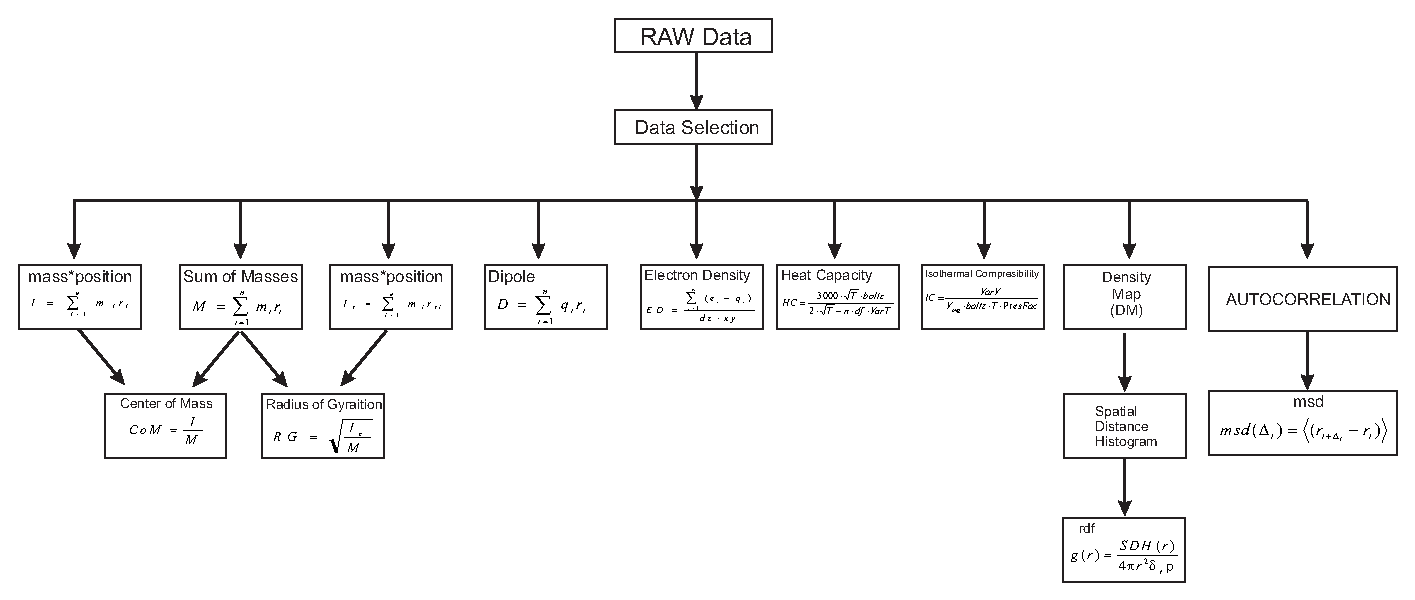
\includegraphics[width=1\textwidth]{images/msstructure.eps} }
 \caption{MS Modules Structure}
 \label{fg:querynetwork}
\end{figure*}


\section{Building the system}\label{sc:system}

\subsection{MS Data retrieval and in memory organization}

A typical MS system generates and stores the data in a number of
trajectory files, usually including multiple frames (snapshots of
the simulated system taken at certain time intervals). Such MS
generated data oftentimes goes through a simple lossless compression
and, depending on the simulation software it may be stored in a
binary format. Such trajectory file format is one of most often used
MS file format (e.g., GROMACS, PDB). But such format is
unrecognizable to our system. So our system has to do three things
before it starts executing the queries: 1) Read the MS data from a
trajectory file, 2) Translate the MS data to a form recognizable to
our system, and 3) Load the data to memory.

\emph{\textbf{Data read - transform.}} As mentioned above, in order
for our system to be able to read the MS generated data, the data
needs to be transformed. The reason for this is following: the MS
data is stored in multiple files and possibly in different formats
as well. One such file holds the global data (identifying the system
and the simulation). Another file holds each frame's data. The frame
data contain general information about the frame, but the main part
is a sequential list of each atom's info, including atom's mass,
position, charge, number of electrons, velocities, forces, etc.
Another file (topology file) holds the molecule/residue info,
essentially identifying what atom belongs to which molecule.

So, in order to extract the data from these files, we have created a
sort of "extractor/transformer" of the attributes needed for the
execution of the queries in our system. This transformer,
essentially, is a separate piece of code that does three things: 1)
it reads the MS generated data that the MS system stores in one of
the often used MS file format (e.g., GROMACS); 2) it translates the
data into a format that our system can read (taking only the
information our system needs); and 3) it stores the data in a file
that has basic structure to it. So, in the end, the data transformer
produces a data file that our system takes as input. This code
serves as a connection between an MS system (e.g., GROMACS) and our
system. With this, our system can essentially be used as an add-on
to GROMACS or other simulation systems and help improve the
efficiency of the data analysis.


\textbf{\emph{Data organization in main memory.}}\footnote{This
paragraph talks only about the data organization used by one-body
queries. For two-body queries (e.g., SDH), the data organization is
discussed later on.} Once the data is in a format our system can
read, the data is being loaded into the main memory one frame at a
time. The organization of the in-memory particle's data is in the
form of a simple, two dimensional array where a single row
represents an atom in the system with all its attributes (e.g.,
coordinates, mass, charge, residue info, etc.). We also keep (in a
one dimensional array) crucial system's information for each frame,
like temperature, energy, pressure, etc. We have used such
structures because they are very suitable for simulating a
push-based type of system: a simple sequential read of the array
gives that on-line type of data stream. So, as the system reads the
array, it pushes the data onto the query-modules. As mentioned
earlier, the one-body (algebraic) queries will produce a final
result at the end of the first sequential read. However, the
two-body (holistic) functions, like SDH and RDF, cannot do this in a
single read of the data.\footnote{However, we have previously
deigned and created a data structure and an algorithm that can take
the advantage of a single data read and produce final results for
SDH computation~\cite{ytu:icde09,EDBT12}. We have incorporate this
into our system presented in this paper.} Therefore, each frame's
data array can be continuously read (in a loop manner) as many times
as a query needs it.
\subsection{Query modules}

As mentioned earlier, there are two types of functions/queries used
for analysis of MS systems: algebraic or one-body, and holistic or
two-body queries (these in general can be multi-body, but in this
paper we only deal with a two-body functions).

\subsubsection{One-body queries} Most of the query modules in
Table~\ref{tb:queries} (except the SDH and RDF) are not that
involved, only containing computations of fairly simple, one-body
functions. These queries were coded as separate modules in our
system. Each of these modules take few attributes as input (e.g.,
atom selection, frames selection(for the autocorrelation functions),
number of atoms, etc.). The system pushes the data as it becomes
available onto these modules. The queries are being executed on the
selection and are put in a ``ready'' mode, awaiting the next frame's
data. First, the more basic queries, like total mass, are being
computed. The results of such queries are temporary stored (in main
memory) and are available for use anytime a more complex query needs
them.

\subsubsection{Two-body queries} In general, queries involving two-body functions are a
bit more complex and cannot provide the final result in a single
data read if a straightforward method is used for their computation.
However, in the proposed system we have incorporated a data
structure and an algorithm for the SDH (also RDF) from our previous
work that is suitable for push-based type of system. In this
subsection we give a brief description of the data structure (DM)
and the algorithm (DM-SDH) designed in~\cite{ytu:icde09, EDBT12} and
implemented in the system proposed in this paper. For more detailed
information, please refer to our previously published work on this
topic~\cite{ytu:icde09, EDBT12}

\emph{\textbf{The data structure.}} The simulation data space is
represented by a conceptual data structure we named Density Map
(DM). The density map splits the simulation space into a grid of
equal size regions (or cells). The cells are cubes in 3D and squares
in 2D\footnote{In this paper, we focus only on the 2D data to
elaborate and illustrate the proposed ideas.} Resolution of a
density map is the reciprocal of the cell size in that density map.
In order to generate higher resolution density map, we split each
cell of the current resolution's grid into four smaller cells of
equal size. This design allows us to use a region
quad-tree~\cite{orenstein:ipl82} to organize density maps of the
same data but with different resolutions. So, essentially, a node in
the quad-tree represents a single cell from the DM. Therefore, a
density map of a certain resolution basically is the set of all
nodes of one level of the tree. Each of the tree nodes records the
cell's location in the density map (coordinates of corner points) as
well as the number of particles in each cell. We name the afore
describe tree the Density-Map tree (DM-tree).

\begin{figure}
 \centerline{ 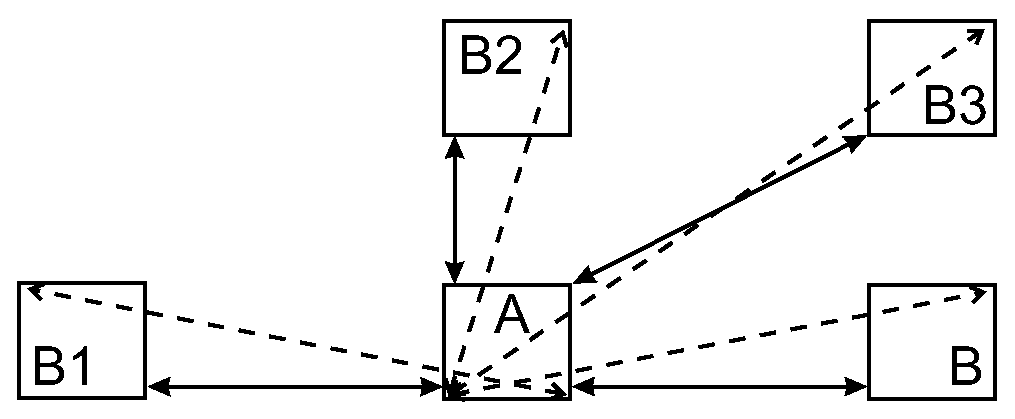
\includegraphics[width=0.65\columnwidth]{images/resolve.eps} }
 \caption{Computing minimum (i.e., length of solid lines) and
 maximum distance (i.e., length of dashed lines) range between two
cells}
 \label{fg:resolve}
\end{figure}

\emph{\textbf{The algorithm.}} The essential part of the DM-SDH
algorithm is a procedure named {\sc ResolveTwoCells}. The input to
this procedure are two cells from the density map (e.g., $A$ and $B$
in Fig.~\ref{fg:resolve}). It computes, in constant time, the
minimum and maximum distance between the two cells. A pair of cells
is ~\emph{resolvable} if both the min and max distance between them
fall into the same SDH bucket $i$. If that is the case, the distance
count of that bucket is being increase by $n_{A}n_{B}$ ($n_{A}$ and
$n_{B}$ are the number of particles in cell $A$ and $B$,
respectively). Otherwise, the cells are non-resolvable and we
either:
\begin{itemize}
\item[(1)] Go to the next density map with higher resolution and resolve all children of $A$
with those of $B$, or
\item[(2)] If leaf-level has been reached: compute every distance between particles of $A$ and $B$ and update the
histogram accordingly.
\end{itemize}

In order to generate the complete SDH, the {\sc ResolveTwoCells}
procedure is executed for all pairs of cells for a given density map
$DM_k$ and the algorithm would recursively call the procedure
(action (1) above) until leaf-level has been reached (action (2)
above).

On top of the aforementioned DM-SDH algorithm, we have also
incorporated two approximate SDH algorithms (ADM-SDH), introduced
and described in \cite{EDBT12}, and \cite{TKDE12}. These approximate
algorithms are substantially faster than the the brute-force
algorithm and also than the DM-SDH algorithm as they take advantage
of some heuristic. For more details on the ADM-SDH algorithms please
see the aforementioned work.


%%%%%%%%%%%%%%%%%%%%%%%%%%%%%%%%%%%%%%%%%%%%%%%%%%%%%%%%%%%%%%%%%%%%%%%%%%%%%%%


\subsection{Working of the system}

In this subsection we give a brief overview of how the system works
at runtime. Please note that the first, preliminary part is only
executed once, i.e., the data transformation from MS data files to a
file that our system can read.

Here are the steps taken through out the analysis:
\begin{itemize}
\item[(1)] Execute the data transformer
\begin{itemize}
\item[(a)] Read the MS data from trajectory files
\item[(b)] Extract the info needed for our system
\item[(c)] Save the read data to a file recognizable to the system
\end{itemize}
\item[(2)] Load the data into main memory (one frame at a time)
\begin{itemize}
\item[(a)] Load data into a double array (for one-body queries)
\item[(b)] Load data into the quad-tree structure (for two-body queries:SDH, RDF)
\end{itemize}
\item[(3)] Push the data to all queries
\item[(4)] A query, if available, acts upon the pushed data (first executing
the lower level, sub-queries)
\item[(5)] Store intermediate results (results
of sub-queries)
\item[(6)] Repeat steps 3-5 if needed.
\item[(7)] Output results
\item[(8)] Go to step 2 and load the next frame (if needed).
\end{itemize}

Fig.~\ref{fg:system} depicts the flow of the system.

\begin{figure}
 \centerline{ 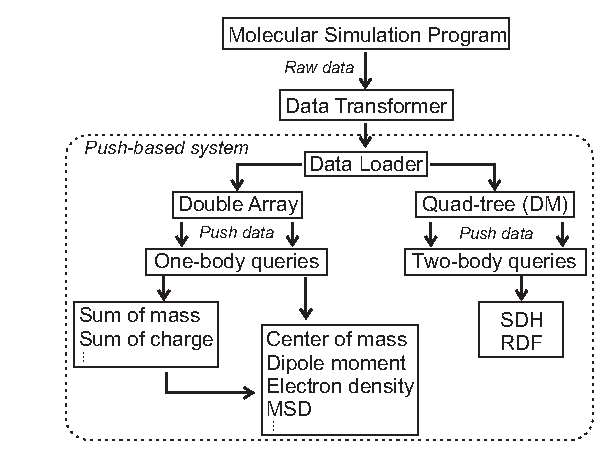
\includegraphics[width=.8\columnwidth]{images/system.eps} }
 \caption{Push-based system flow}
 \label{fg:system}
\end{figure}

Step 2, loading the data into main memory is different for SDH query
compared to the one for the one-body queries. The reason for that,
as mentioned earlier, is the different data structure used to store
the data in memory. While we use double array to store the data for
the one-body queries, we use quad-tree like data structure to store
the data needed to compute the SDH. The loading to the double array
is straightforward. However, to load the quad-tree structure, we
need to use some of the info from the data itself. Namely, the
coordinates of the atoms are used to determine in which tree node an
atom belongs. That way we build the so called density map (DM),
i.e., the different regions with a certain number of atoms in them
(including all the atom's attributes). So basically, to solve the
SDH problem in a push-based manner, we convert the problem into
populating a data structure in push-based manner. This data
structure will then be used as an input to our DM-SDH algorithm
that, although not completely in ``on-the-fly" way, is a great
improvement over the naive methods used in much of today's MS
analysis systems (i.e., GROMACS, PDB, CHARMM, etc.).


%%%%%%%%%%%%%%%%%%%%%%%%%%%%%%%%%%%%%%%%%%%%%%%%%%%%%%%%%%%%%%%%%%%%%%%%%%%%%%%
\begin{figure}
 \centerline{ 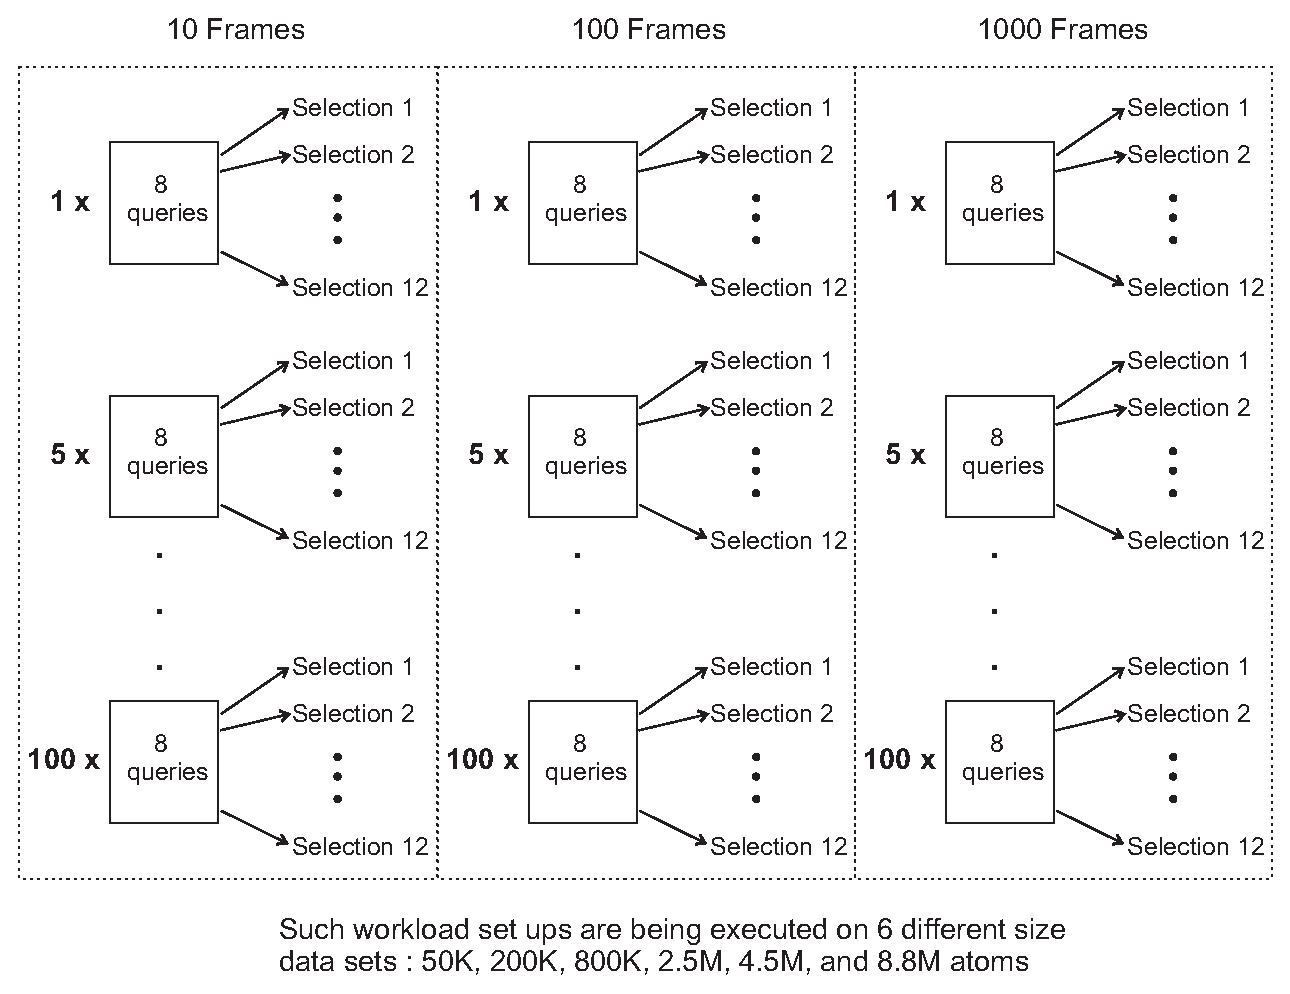
\includegraphics[width=.99\columnwidth]{images/workload_set_up1.eps} }
 \caption{Workload setup}
 \label{fg:workload_set_up}
\end{figure}

\section{Experimental results}\label{sc:experiments}

The system was implemented in C++ programming language and tested on
real molecular simulation data sets. The experiments were carried
out on an Apple MacPro machine with 8GB of physical memory and two
Quad-Core Intel Xeon 3GHz processors. The MacPro was running OS X
Mavericks $10.9.3$ operating system. We have compared the results
obtained by our system to those obtained by running the analysis
through GROMACS (v. $4.5.7$). Both systems were analyzing the same
data sets.

\emph{\textbf{Data sets.}} In our experiments, six data sets from
different simulations were used. All simulations were done on a
POPC~\footnote{POPC is a chemical compound composed of a
diacylglycerol and phospholipid. Its full name is
1-palmitoyl-2-oleoyl-sn-glycero-3-phosphocholine and it is one of
the most important lipids in bio-physical molecular simulation.}
lipid bilayer, but were all set to produce data of different sizes
(i.e., different number of particles in the simulation). Namely, we
have tested the system on simulations with $52,400$; $209,600$;
$838,400$; $2.5M$; $4.4M$; and $8.8M$ atoms. Also, since the
simulations were run separately, they produced six different MS
systems with distinct characteristics (distinct structure, atom's
positioning, etc.). From all of the generated data sets we have
randomly selected sets of $10$, $100$, and $1000$ consecutive frames
for the purpose of our experiments. This gave us $18$ different
datasets on which we tested our system.

\emph{\textbf{Query work load.}} Two types of query workload were
used: 1) one involving one-body queries only 2) one including
two-body queries (SDH and RDF) as well. The reason for this is that
GROMACS, the system we used to compare our system to, only has a
naive method of solving the RDF (SDH) problem (like almost all MS
analysis systems). In our system we have incorporated SDH (RDF)
algorithms that are far more superior to the naive method, and
comparing the systems like that would not have been fair (we
believe).

\emph{\textbf{One-body queries only.}} The following set of one-body
queries were included in the test workload: mean square displacement
(msd), radius of gyration, dipole moment, center of mass, velocity
autocorrelation, electron density, mass density, and charge density.
This set of queries were pointed to us, by a group in the physics
field with extensive MS background, as one of the most commonly used
in the field of collagen bilayer MS system analysis. A workload
group contains all $8$ queries executed on one of the $12$
selections, making $12$ groups. Such groups are executed on six
different size data sets, with $10$, $100$ and $1000$ frames. This
workload is then repeated $5$ more times, by executing each of the
queries in the groups $5$, $10$, $25$, $50$, and $100$ times,
essentially just magnifying the workload intensity. In total, we
have $12 x 6 x 3 x 6 = 1,296$ different workload setups to test the
system on. Fig.~\ref{fg:workload_set_up} shows the organization of
the workload setup.

%%%%%%%%%%%%%%%%%%%%%%%%%%%%%%%%%%%%%%%%%%%%%%%%%%%%%%%%%%%%%%%%%%%%%%%%%%%%%%%

\subsection{Benchmark}

Through extensive collaboration with a research group from the
Physics department at USF, we have come up with a benchmark that can
be used for testing the efficiency of an analysis system for
molecular simulations. The benchmark consist of three essential
parts: 1. Simulation data produced by an MS, 2. Queries that are to
be executed onto that data in order to produce some information of
interest, and 3.Benchmark parameters that control the size of the
benchmark.


\subsubsection{Benchmark Data}
The data used in the benchmark was real molecular simulation data,
produced through the GROMACS MS system. The initial, pre-simulation
data file consisted of $200$ POPC and $12000$ solvent molecules, or
$12200$ molecules in total. This type of system was used because it
is sufficiently diverse, containing enough distinct POPC and solvent
molecules (e.g., each POPC molecule includes approximately $52$
different atoms) and yet simple enough to be easily transformed into
another system of different size. By using the $genconf$ function in
GROMACS, we produced pre-simulation files of different sizes
(essentially by changing the system's size (box)). $Six$ different
sized pre-simulation files were created. A molecular simulation was
then run on these $6$ files, each producing an MS system of certain
size (volume/number of particles). All of the simulations were set
up to produce $1000$ frames (snapshots in time of the systems), each
frame containing the same number of particles as the base one. The
produced files contained: $52,400$; $209,600$; $838,400$; $2.5M$;
$4.4M$; and $8.8M$ atoms per frame. So, for example, the file with
$52,000$ atoms holds $52,000,000$ records in total ($1000$ frames,
each containing $52,000$ records). As mentioned earlier, this
simulation data comes mostly in binary formats and in trajectory
files having a lot of unneeded overhead. Therefore, it was
transformed to a data arrays files containing only crucial
information of the particles and the system. The size of the files
ranged from $135MB$ for $52,000$ atoms to $24GB$ for $8.8$ million
atoms (this is for data with $100$ frames).

%Fig.~\ref{fg:dataformat} represents the organization/structure of
%these files.

\subsubsection{Benchmark Queries}
The queries selected to be included in this benchmark were derived
through a thorough observation of the way an MS system is being
analyzed. They were found to be the base of the analysis of many MS
systems. In other words, no mater how small or big the analysis was,
these queries were included in that analysis. As mentioned earlier,
they are of two types: one-body (and algebraic) and two-boy (and
holistic). Table~\ref{tb:queries} shows these queries.


\subsubsection{Benchmark Parameters} There are several parameters
that can be used to control the overall size of the system. We divide the parameters into two groups:\\
Data size parameters:
\begin{itemize}
\item[-]Select different sized dataset
\item[-]Number of frames
\item[-]Data selection (within the selected dataset) onto which the queries are being executed
\end{itemize}
Workload size parameters:
\begin{itemize}
\item[-]Number of queries to be executed
\item[-]Number of times each query is executed
\end{itemize}
By changing these parameters, we can produce a versatile testing
benchmark for MS analysis systems.

%%%%%%%%%%%%%%%%%%%%%%%%%%%%%
\begin{comment}

\begin{figure}
 \centerline{ 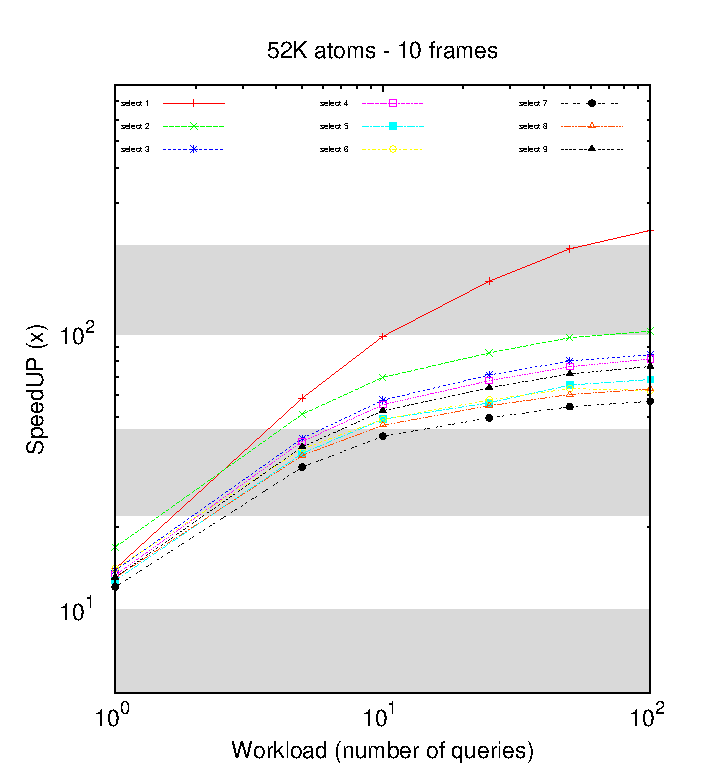
\includegraphics[width=columnwidth]{images/speedup10frames52K.eps} }
 \caption{Showing speedup for different workload}
 \label{fg:results2-10frames}
\end{figure}

\begin{figure}
 \centerline{ 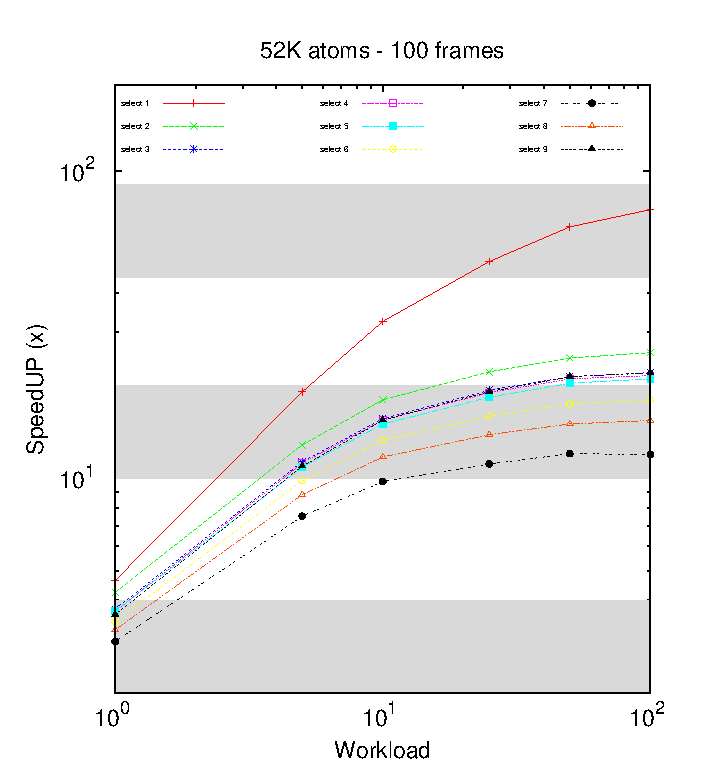
\includegraphics[width=columnwidth]{images/speedup100frames52K.eps} }
 \caption{Showing speedup for different workload}
 \label{fg:results2-100frames}
\end{figure}

\begin{figure}
 \centerline{ 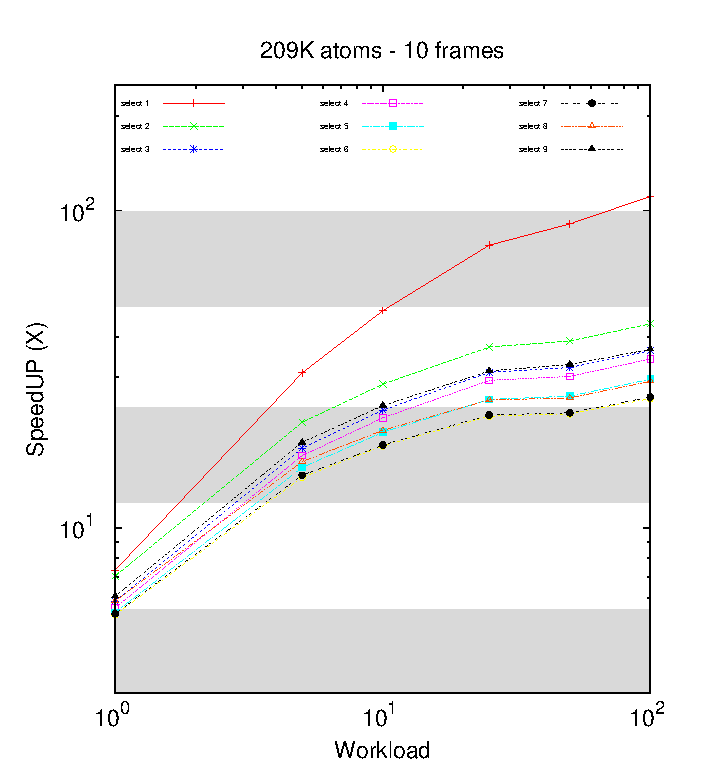
\includegraphics[width=columnwidth]{images/speedup10frames209K.eps} }
 \caption{Showing speedup for different workload}
 \label{fg:results3-10frames}
\end{figure}

\begin{figure}
 \centerline{ 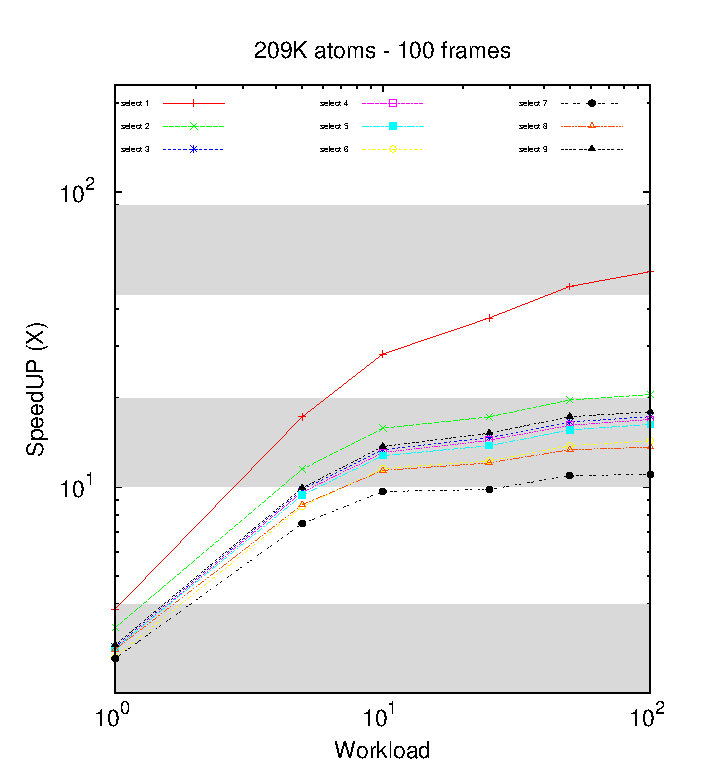
\includegraphics[width=columnwidth]{images/speedup100frames209K.eps} }
 \caption{Showing speedup for different workload}
 \label{fg:results3-100frames}
\end{figure}

\end{comment}
%%%%%%%%%%%%%%%%%%%%%%%%%%%%%%%%%%%%%5


%\begin{figure}
% \centerline{ 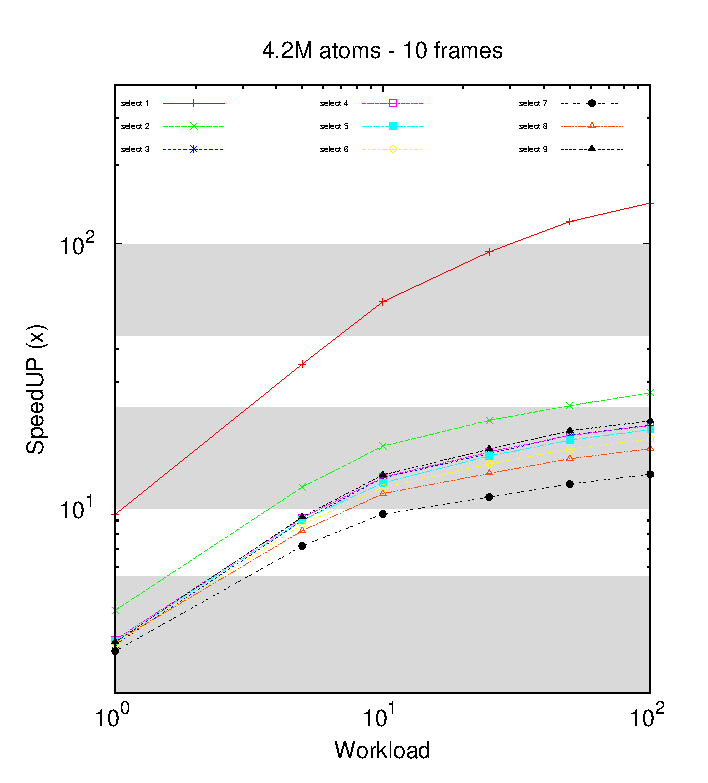
\includegraphics[width=.8\columnwidth]{images/speedup10frames4.2M.eps} }
% \caption{Showing speedup for different workload}
% \label{fg:results5-10frames}
%\end{figure}

\subsection{Results} We have run extensive experiments over all the
different setups of workload mentioned previously in this section.
However, in this paper we present only the workload setups of $4$
data size sets: $838,400$, $2.5M$, $4.2M$, and $8.8M$ atoms because
we believe they convey enough information about the efficiency of
our system compared to that of the Gromacs system. The running times
of our push-based system were compared to those of the Gromacs
system. The first set of figures, namely
Figures~\ref{fg:speedup838K-select-level}-\ref{fg:speedup8.8M-select-level},
represent the speedup that our system obtains over the Gromacs
system with various atoms selection levels. We define the selection
levels based on the number of comparisons we have to make in order
to extract the needed group(selection) of atoms. For example, if we
want to do analysis on all molecules containing oxygen, or hydrogen,
or carbon we would go over each molecule and compare its components
to the selection list. The bigger the selection list, the higher the
select level in our system. For better visualization, we note three
different selection levels: high (at least $10$ comparisons made),
medium (between $1$ and $10$ comparisons made), and low select level
(with one or less comparisons made). As seen in the figures, for
high selection level, the speedup is smaller compared to that
achieved in low select levels. The reason for this, we believe is in
that the amount of time our system spends extracting the atoms group
increases with the level of selection. Even though our system still
shows considerable speedup over Gromacs in high level selections, we
do believe there is room for improvement in our system and that is
our immediate future work we are planning on doing. These figures
also show the relation of the speedup to the workload intensity,
i.e., the higher the workload intensity the higher the speedup.

The connection between the workload intensity and the speedup is
better represented in the next set of figures,
Figures~\ref{fg:speedup838K}-\ref{fg:speedup8.8M}. They show the
speedup our system achieves over the Gromacs system on a varying
workload intensity. Each of those figures show the speedup with
different dataset sizes (e.g., $838,000$, $2,567,600$ atoms, etc.),
including $10$, $100$, and $1000$ data frames. The speedup is
calculated simply as a ratio between the running time of our system
on a certain set of workload and that of the Gromacs system on the
same workload. These figures show that the speedup over varying
workload intensity achieved by our system ranges anywhere from about
$10$ to $1000$ times, depending on the size of the dataset, number
of frames and the selection of the atoms.

Figure~\ref{fg:speedup-average-over-all-workload}, shows the speedup
our system achieves over all workload intensity (average workload
intensity) with varying dataset sizes. It is clear that, again our
system has better performance than the Gromacs system. The speedup
presented in this set of figures ranges anywhere from about $15$ to
$650$ times.


The last figure, Figure~\ref{fg:speedup-average-workload-select},
shows the speedup our system achieves over all workload intensity
and all select levels with varying dataset sizes. This figure, in a
way, summarizes the previous two sets of figures, bringing together
the workload and the different selections through the average. It is
clear that, again our system has better performance than the Gromacs
system. The speedup ranges anywhere from $50$ to $250$.

All four sets of figures show that such push-based design has clear
advantages over the pull-based type of design incorporated in the
Gromacs system.



\section{Conclusions and Future Work}\label{sc:conclusion}
The objective of our work is to design and implement improved data
analysis system that can be used in the field of molecular
simulation system's analysis. In this paper, we introduce the idea
for such system. We build our system on a push-based type design,
where data from data arrays is being pushed onto available queries
in the system. These queries are being executed on the pushed data
and produce intermediate / final result that would be used as part
of the data analysis. We are able to achieve an improvement over
existing, pull-based type designs because of the I/O overhead such
designs introduce when dealing with large volumes of scientific
data. Also, our queries are able to be executed on the same stream
of data, making it suitable solution for streaming circumstances. We
designed a benchmark that can be used to test data analysis systems.
This benchmark comprises of three parts: 1)benchmark data,
2)benchmark queries, and 3) benchmark parameters. We use this
benchmark to compare our system to one of the most frequently used
MS analysis systems, Gromacs. The efficiency and speedup achieved by
our system is supported by extensive experiments and their results.
The results show that our push-based design achieves up to about
$1000$ times speedup in comparison to a pull-based design, i.e.,
Gromacs.

One direction of our future work will be to further improve our
push-based design. Through the extensive experiments we have learned
that our design can be improved when the atom selection clause
involves many conditions. This improvement may be in the direction
of improving the algorithmic part, but it can also be in the
direction of improving the data presentation/organization we have
used in the system.\\

%%%%%%%%%%%%%%%%%%%%%%%%%%%%%%%%%%%%%%%%%%%%%%%%%%%%%%%%%%%%%%%%%%%%%%%%%%%%%%%


\noindent{\bf Acknowledgements:} The project described was supported
by an Award (R01GM086707) from the National Institute Of General
Medical Sciences (NIGMS) at the National Institutes of Health (NIH).
The authors would like to thank Anand Kumar who has contributed his
time and knowledge toward completion of the work.


%%%%%%%%%%%%%%%%%%%%%%%%%%%%%%%%%%%%%%%%%%%%%%%%%%%%%%%%%%%%%%%%%%%%%%%%%%%%%%%
%%%%%%%%%%%%%%%%%%%%%%%%%%%%%%%%%%%%%%%%%%%%%%%%%%%%%%%%%%%%%%%%%%%%%%%%%%%%%%%
%%%%%%%%%%%%%%%%%%%%%%%%%%%%%%%%%%%%%%%%%%%%%%%%%%%%%%%%%%%%%%%%%%%%%%%%%%%%%%%


\bibliographystyle{IEEEtran}
\bibliography{push-based-MS}
\begin{comment}
\begin{IEEEbiographynophoto}{Vladimir Grupcev}
received a BS degree in Applied Mathematics \& Computer Science from
University of Ss. Cyril and Methodius, Macedonia in 2005; Master's
degree in Mathematics from University of South Florida in 2007. He
is currently a PhD student in the department of Computer Science \&
Engineering at the University of South Florida. His area of interest
includes scientific data management and high performance computing.
\end{IEEEbiographynophoto}
\vspace{-10mm}
\begin{IEEEbiographynophoto}{Yi-Cheng Tu}
received a Bachelor's degree in horticulture from Beijing
Agricultural University, China, and MS and PhD degrees in computer
science from Purdue University (2003; 2007). He is currently an
assistant professor in the department of Computer Science \&
Engineering at the University of South Florida. His research is in
energy-efficient database systems, scientific data management, high
performance computing and data stream management systems.
\end{IEEEbiographynophoto}
\vspace{-10mm}
\begin{IEEEbiographynophoto}{Sagar Pandit}
Dr. Sagar Pandit is an Assistant Professor of Physics at the
University of South Florida. He received his Ph.D. from the
Department of Physics, University of Pune, in 1999 in the area of
Dynamical systems. Later, his research shifted to Biological
Physics, specifically membrane physics. His current research
interests include  biomembranes, mathematical modeling of complex
biological and social systems, dynamical systems, and computational
approaches toward addressing problems in these fields.
\end{IEEEbiographynophoto}
\end{comment}

% if you will not have a photo
%\begin{biographynophoto}{John Doe}
%Biography text here.
%\end{biographynophoto}

% insert where needed to balance the two columns on the last page

\clearpage

%%%%%%%%%%%%%%%%%%%%%%%%%%%%%%%%%%%%%%%%%%%%%%%%%%%%%%%%%%%%%%%%%%%%%%%%%%%%%%%
%%%%%%%%%%%%%%%%%%%%%%%%%%%%%%%%%%%%%%%%%%%%%%%%%%%%%%%%%%%%%%%%%%%%%%%%%%%%%%%

\appendices

%%%%%%%%%%%%%%%%%%%%%%%%%%%%%%%%%%%%%%%%%%%%%%%%%%%%%%%%%%%%%%%%%%%%%%%%%%%%%%%

\end{document}
